\section{Usability Test}
\label{common:sec:usability_test}
%FORM�L
	%Hvad er form�let med en brugevenlighedstest
	%Hvorfor har vi valgt at have det med?
	%Integrationstest, h�nger de forskellige dele sammen for brugeren
	%Individuelle form�l
%The system description \ref{common:sec:sys_description} states, that GIRAF is a collection of applications for Android designed for use by children with autism spectrum disorder. %Gentagelse af noget der kommer to afsnit tidligere, kan eventuelt udelades
The usability of GIRAF is important because GIRAF is supposed to be a tool the guardians can use on a daily basis in interaction with children.
GIRAF is built as an alternative to the tools guardians already use when working with children.
Therefore is it important that the guardians want to pick GIRAF instead of the tools they already have.
This requires GIRAF to be a system the guardians can learn to use quickly and a tool the guardians feel comfortable with.\\
\\
The usability test is also a good indicator of how the individual applications are integrated with each other.
As a developer in a development environment the applications you make, may seem like they are integrated very well.
But when introduced to the real world, the user might find that the applications aren't working together at all.

\subsection{Approach}
%FREMGANGSM�DE
		%INVITATION
		%Reference til appendix
The most obvious test group was the persons already involved with the project as contacts.
The invitation sent to the test persons can be found in the appendix \ref{appendice:usability_test}.\\

Since the main focus of the project is not the usability, the purpose of the test is to recognize the most critical usability errors and not to acknowledge all errors of the application.
Because of this would a test method which favors that there is no need to spend a lot of time on usability testing, be the best choice.
Furthermore is the amount of test persons relatively small, approximatly 4-6 persons.
Based on the fact that the test should be short and the test group is small, the Instant Data Analysis method for usability testing is perfect for the GIRAF project \cite{usability:ida}.

\subsubsection*{Setup}
	%OPS�TNING
		%Billede og beskrivelse af hvordan det foregik
		%Optagelser, video + lyd - hvorfor?
		%Hvilke opgaver/personer var med til testen?
The usability test is divided into two tests, a test of the three applications and a test of the two administrations applications (Android and web).
Each test is assigned a team to accommodate the need to run two tests simultaniously.
The teams are made with respect to the criteria of the Instant Data Analysis process.\\
Each team consisting of at least:

\begin{itemize}
	\item 1 x Test Coordinator
	\item 1 x Test Monitor
	\item 1 x Data Logger
\end{itemize}

To ensure that as many errors has been recognized as possible were the three mandatory persons assisted by two observers.\\
\\

The usability lab on Aalborg University is designed with two rooms for usability testing and a control room to observe and record the tests.
The two test chambers were assigned a test each and the control room were used to observe both tests as seen in figure \ref{fig:test_setup}.

\begin{figure}[H]
	\centering
		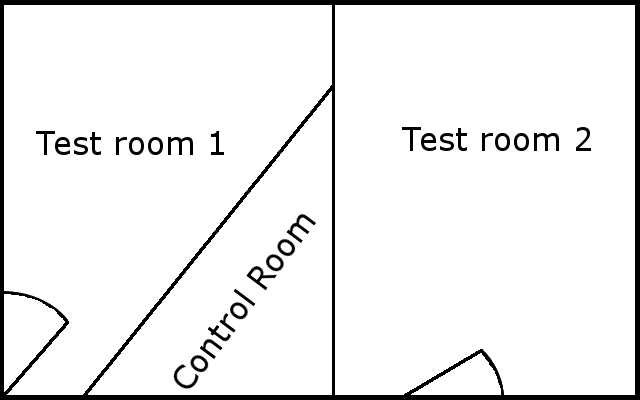
\includegraphics{images/test_setup.png}
	\caption{An overview of how the usability lab on Aalborg University.}
	\label{fig:test_setup}
\end{figure}

All tests were recorded on video and audio as well as documented for later analysis.

\subsubsection*{Execution}
%UDF�RSEL
		%Hvordan gik det til?
		%Modtagelse
		%Briefing
		%Test + debriefing
To ensure an even experience of the test for all users, each test person was introduced in the same manner by the Test Coordinators.
The Test Coordinators briefed and the interviewed the test persons before each test.
Furthermore did the Test Coordinators debrief and interview the test persons along with a questionnaire after each test to get an understanding of their opinion of the system.\\
The documentation of this can be found in appendice \textcolor[rgb]{1,0,0}{Ved ikke hvor det er og hvor det skal v�re?}.\\
\\

The two test teams used the Instant Data Analysis method to evaluate on the usability tests and give the final result of the tests.
The test results can be found in section \textcolor[rgb]{1,0,0}{Inds�t reference} in the individual part of the report.
	%EVALUERING
		%Instant data analysis
		
%RESULTAT - IKKE F�LLES